\documentclass{article}

%\usepackage[margin=3.7cm]{geometry}
\usepackage[utf8]{inputenc} 
\usepackage[T1]{fontenc}
\usepackage[brazil]{babel}
\usepackage{mathtools, amssymb} %{amsmath}
\usepackage{amsmath}
\usepackage{float}
\usepackage{graphicx}
\usepackage{wrapfig}
\usepackage[style=brazilian]{csquotes}
\usepackage[dvipsnames]{xcolor}
\usepackage{complexity}
\usepackage{diagbox}
\usepackage{amsfonts}
\usepackage{algorithm,algpseudocode}


% TODO: Apagar
\usepackage[colorinlistoftodos, color=yellow]{todonotes}

\setlength{\parskip}{1em} %espaço entre os parágrafos%

\graphicspath{ {Imagens/} }

\algnewcommand{\algorithmicand}{\textbf{ and }}
\algnewcommand{\algorithmicor}{\textbf{ or }}
\newcommand{\algorithmicbreak}{\textbf{break}}
\algnewcommand{\OR}{\algorithmicor}
\algnewcommand{\AND}{\algorithmicand}
\newcommand{\BREAK}{\State \algorithmicbreak}


\begin{document}
	\begin{wrapfigure}{L}{0.3\textwidth}
		\begin{flushleft}	
			
\includegraphics[height=.065\textheight]{PESC.png}
		\end{flushleft}
	\end{wrapfigure}
	
	\quad\\
	{Universidade Federal do Rio de Janeiro} \\
	{Otimização Combinatória - COS890} \\
	{Professor: Abilio Lucena}
	
	\quad\\
	\vspace*{2cm}
	
	\begin{center}
		\huge\bfseries
		Leilões Combinatórios - uma aplicação do problema de empacotamento de conjuntos através de métodos exatos
	\end{center}
	\vspace*{3mm}
	
	\begin{center}
		\large
		Amanda Camacho Novaes de Oliveira
		
		Diego Amaro Ferraz da Costa	
		
		Diego Athayde Monteiro 
	\end{center}

	\vspace{1cm}
	
	
	\begin{abstract}
	    Neste trabalho, descrevemos o problema dos leilões combinatórios como uma aplicação do \textsc{problema de empacotamento de conjuntos}, um conhecido problema proposto por Karp \cite{Karp}. Aplicamos três algoritmos exatos para a resolução do mesmo através do solver \emph{Gurobi}, utilizando a linguagem de programação \emph{Julia} e biblioteca \emph{JuMP} que nos fornece muitas ferramentas úteis para a resolução de problemas de otimização. Utilizamos duas bases de dados com instâncias de diferentes tamanhos e comparamos os resultados obtidos por cada um dos métodos exatos que descrevemos aqui, sendo estes: uma relaxação lagrangeana, um algoritmo \emph{branch and bound} e um algoritmo \emph{branch and cut}.    
	 \end{abstract}
	
	
	
	\section{Introdução}
	A otimização combinatória representa uma área da ciência da computação e de matemática aplicada que estuda problemas de otimização em conjuntos finitos. Os problemas de otimização são aquelas onde se procura determinar valores extremos de um conjunto de restrições, com respeito a uma função, esta chamada de função objetivo. As variáveis envolvidas nos problemas de otimização são denominadas variáveis de decisão. Quando falamos destas variáveis, podemos dividir os problemas de otimização em duas categorias: problemas onde as variáveis são lineares e problemas onde elas são não lineares. E ainda podemos fazer mais uma distinção quanto aos problemas de otimização combinatória que estamos lidando, e esta distinção é através dos valores que as variáveis podem assumir. Podemos ter problemas onde as variáveis podem assumir valores reais, inteiros, binários ou ainda um misto destas classificações.
	
	Neste trabalho, definimos e aplicamos técnicas de soluções exatas para um conhecido problema, onde as variáveis são lineares e podem assumir valores binários 0-1. Este problema é o \textsc{problema de empacotamento de conjuntos}. Mais especificamente, sua versão de otimização.
	O problema consiste em: dado um cojunto finito $I$ de $n$ elementos e um conjunto finito $J$ de $m$ elementos, desejamos obter o conjunto $I_j$ dos subcojuntos viáveis (a cada um destes subconjuntos é associado um peso $c_j$) de $I$ com o maior peso possível. Vamos definir de maneira mais formal, detalhar o problema e sua formulação em uma seção mais adiante.
	
	Este problema possui muita aplicação prática e uma das mais conhecidas é a de Leilões Combinatórias que é abordagem que fazemos neste trabalho. Um leilão combinatório consiste em distribuir um número $m$ de produtos através de $n$ lances. Se um lance é escolhido, um determinado lucro é obtido. O objetivo em um leilão combinatório é maximizar o lucro total respeitando a condição de que cada produto só pode estar contido em no máximo um lance. Utilizando esta aplicação do \textsc{problema do empacotamento de conjuntos}, utilizamos três métodos exatos para resolver o problema: uma relaxação lagrangeana, um algoritmo \emph{branch and bound} e um segundo algoritmo \emph{branch and bound} com algoritmos de planos de corte associados ao mesmo, denominado \emph{branch and cut}.
	
	Esse texto está organizado da seguinte forma: na seção~\ref{sec:prob}, detalhamos o \textsc{problema de empacotamento de conjuntos}, na seção~\ref{sec:caso} exibimos um caso base do problema e nas seções \ref{sec:relag}, \ref{sec:BB} e~\ref{sec:BC} descrevemos um pouco cada método aplicado e por fim nas seções~\ref{sec:res} e~\ref{sec:disc} exibimos os resultados obtidos e a comparação entre os mesmos e por fim, na seção~\ref{sec:concl} nossas conclusões e ideias para trabalhos futuros.
	
	
	\section{O Problema de Empacotamento de Conjuntos}\label{sec:prob}
	O \textsc{problema de empacotamento de conjuntos} (do inglês, Set-Packing Problem) foi um dos 21 problemas enunciados por Karp em \cite{Karp}. Neste mesmo trabalho, Karp mostrou que se trata de um problema \NP-completo através de uma redução feita do \textsc{problema da clique máxima de um grafo}. O \textsc{problema de empacotamento de conjuntos} também possui forte relação com o \textsc{problema da cobertura de conjuntos}, problema este que é o dual do problema aqui tratado.
	
	A versão de decisão consiste em determinar, dado um inteiro $k$, se existe um conjunto com $k$ subconjuntos do conjunto de subconjuntos viáveis $I_j$. Porém, neste trabaho, abordamos a versão de otimização, descrita a seguir.
	
	A descrição formal do problema é dada da seguinte forma:
	
	\begin{itemize}
	    \item[-] $I$ = \{1, ..., m\}: conjunto finito de elementos
	    
	    \item[-] $J$ = \{1, ..., n\}: conjunto finito de índices
	    
	    \item[-] \{$I_j$ $\subseteq$ : $j$ $\in$ $J$\}: conjuntos dos subconjuntos viáveis de $I$
	    
	    \item[-] Existe um peso $c_j$ à cada $I_j$, $j$ $\in$ $J$
	    \{$I_j$ $\subseteq$ : $j$ $\in$ $J$\}: conjuntos dos subconjuntos viáveis de $I$
	    
	    \item[-] \{$I_j$ : $j$ $\in$ $J_i$\}: subconjuntos dos subconjuntos viáveis de $I$ que contém $i$~$\in$~$I$
	    \item[-] Variáveis binárias $x_j$ $\in$ \{0,1\} que expressam a decisão de escolher ou não $I_j$, $j$~$\in$~$J$
	\end{itemize}
	
	
	Por fim, sua formulação como um problema de programação inteira é:
	
	\begin{equation*}
        \begin{array}{ll@{}ll}
            \text{max}  & \displaystyle\sum\limits_{j \in J} c_{j}&x_{j} &\\
            \text{sujeito a}& \displaystyle\sum\limits_{j \in J_i}   &x_{j} \leq 1,  &i \in I\\
                 &                                                &x_{j} \in \{0,1\}, &j \in J
        \end{array}
    \end{equation*}
    
	Este problema possui uma ampla aplicação prática. Como um exemplo destas, temos o escalonamento de tripulações de companhias aéreas para aviões. Cada avião da frota precisa ter uma tripulação designada a ele, composta por um piloto, copiloto e navegador~\cite{Airline}.    
    Como mencionado anteriormente, a abordagem que fazemos aqui ao \textsc{problema de empacotamento de conjuntos} é feita no contexto dos leilões combinatórios, que é objeto de estudo de muitos estudiosos em diversos trabalhos (\cite{Winner}, \cite{Taming}, \cite{CABOB}). Nesta aplicação os conjuntos $I$ e $J$ podem ser enxergados como um conjunto de $m$ produtos e um conjunto de $n$ lances, respectivamente. Nosso objetivo então é: maximizar o lucro total obtido sem violar a restrição de que um produto só pode ser escolhido por, no máximo um lance. E este lucro é um valor associado a seleção de cada produto. 

    \todo[inline]{Adicionar nossa forma de aproximação do problema}
	
	\section{Relaxação Lagrangeana}\label{sec:relag}
	A relaxação lagrangeana consiste em um método de decomposição das restrições de um determinado problema em dois grupos: as restrições "convenientes" e as restrições "inconvenientes". De tal forma que as restrições "incoveninentes" são retiradas do problema de programação inteira e adicionadas à função objetivo em um termo $u(d - Dx)$. Estas variáveis $u_i$ são denominadas variáveis duais ou multiplicadores de Lagrange.
	
	De fato, nem sempre a relaxação lagrangeana nos oferece uma solução ótima para o problema. Porém, mesmo nos casos em que a solução obtida não é ótima, podemos extrair informações interessantes ao interpretar o resultado obtido.
	O segundo grupo de restrições, as "convenientes" tornam o problema mais fácil de ser resolvido e eventualmente podemos obter a solução ótima para o problema original através da relaxação.
	
	O ponto de partida para a aplicação deste método é a elaboração do subproblema lagrangeano. Baseado no modelo de programação inteira que apresentamos na seção~\ref{sec:prob}, o subproblema lagrangeano para o \textsc{problema de empacotamento de conjuntos} é: 
	
	\begin{equation*}
        \begin{array}{ll@{}ll}
            \text{max}  & \displaystyle\sum\limits_{j \in J} (c_{j} - \displaystyle\sum\limits_{i \in I_j} u_{j})x_j+  \displaystyle\sum\limits_{i \in I} u_{i}\\
            \text{sujeito a}
                 &                                                x_{j} \in \{0,1\}, j \in J
        \end{array}
    \end{equation*}
	
	\todo[inline]{Descrição do algoritmo Lagrangeano (pseudo-código do que implementamos). Critérios de parada}
	 
	% \begin{algorithm}
    %     \caption{Subgradiente para o problema de empacotamento de conjuntos}
    %     \begin{algorithmic}[1]
    %         %\Statex \textbullet~\textbf{Parameters:} $n, t \in % \mathbb{N}$, where $t < n$.
    %         \State \For{$k = 0$, $k < $maxInt, $ k++$}
    %         \State $z_u$, $x_u$ = limite\_superior()
    %         \State $z_l$, $x_l$ = limite\_inferior()
    %         
    %         
    %         \State Second step
    %         \State \ldots
    %     \end{algorithmic}
    % \end{algorithm} 
	
	\begin{algorithm}
    \caption{Subgradiente para o problema de empacotamento de conjuntos}
        \begin{algorithmic}[1]
            \Statex \textbullet~\textbf{Parameters:} $n, t \in \mathbb{N}$, where $t < n$
            \State Variáveis:
            \State MaxIter := Número máximo de iterações definido
            
            \State s = zeros(m), sqrSum = 0, $\pi_{min}$ = 0.0001
            
            \State $k = 0$ \Comment{{\color{gray} Índice da iteração}}
            
            \State Definir $\pi = 2$ e multiplicadores de Lagrange $u = 0$
            
            \State Resolver o subproblema Lagrangeano, obtendo: $\overline{x}$, $\overline{z}$
            
            \State $k := k + 1$
            \State \If {$k = $ MaxIter}  
            \State \Return PARE
            \State \EndIf
            \State \If {$\overline{z} - \underline{z} < 1$}  
            \State \Return \underline{x} \Comment{{\color{gray} Valor ótimo encontrado}}
            \State \EndIf
            \State \If {$\overline{z} = \underline{z}$}  
            \State \Return o valor ótimo encontrado
            \State \EndIf
            %\underline{}
            
    
            \Statex
            \Statex Cálculo do tamanho do passo: 
            \State 
            \For{cada produto $i$}
            \State $s[i] = 1 - \sum_{j\in L} a[i,j]*\overline{x}[j]$
            \State $u_i = \max \{0,(1+ \epsilon) T \cdot s_i\}, \quad \forall i= 1,\dots,m$
            \State sqrSum = sqrSum + $s[i]^2$
            \EndFor
            \State $T = \dfrac{\pi * (\overline{z} - \underline{z})}{sqrSum} $
            \State \If{$T < \pi_{min}$}
            \State \Return valor do t muito pequeno - PARE
            \State \EndIf
            \State retornar para a linha ....
    
    
            \Statex
            \Statex Critérios de Parada do Código
            
    
    
        \end{algorithmic}
    \end{algorithm}
	
	
	\section{Branch and Bound}\label{sec:BB}
	Uma técnica muito aplicada para resolução de problemas combinatórios é a técnica de dividir e conquistar que consiste em resolver subproblemas mais fáceis que o original e após este processo combinar as soluções obtidas até obtermos a solução do problema original. Porém, esta enumeração de subproblemas de forma explícita pode ser muito custosa, e justamente neste contexto, é que algoritmo \emph{Branch and Bound} entra em ação.
	
	O algoritmo \emph{Branch and Bound} consiste em uma técnica de enumeração implícita de soluções, onde através de limites locais, obtemos limites globais. Toda a eficiência e ganho que o algoritmo \emph{Branch and Bound} nos oferece é por conta das podas que acontecem na árvore de enumeração implícita, que podem ocorrer por: otimalidade, inviabilidade e limites duais. A técnica foi definida primeiramente em~\cite{Land} por Ailsa Land e Alison Doig em 1960, e figura como um dos mais importantes métodos exatos no contexto de resolução de problemas de otimização até os dias atuais.
	
	
	
	\section{Branch and Cut}\label{sec:BC}
	Para fortalecermos ainda mais o algoritmo \emph{Branch and Bound}, é possível utilizarmos de algoritmos de planos de corte para em cada nó de sua árvore de enumeração. % NOTE: COPIA
	Assim sendo, antes de efeturamos o \emph{Branching} de um determinado nó, tentamos fortalecer os limites duais através de planos de corte. 
	
	Ao invés de reotirmizarmos rapidamente em cada nó, a ideia consiste em gastar mais tempo em cada nó, na esperança de haver um ganho global, possivelmente, em número de nós explorardos e em tempo de CPU. % END COPIA
	
	Como desiqualdades válidas para o \textsc{problema de empacotamente de conjuntos}, utilizamos desigualdades de cliques geradas a partir de um grafo conflito. Este grafo é definido da seguinte forma: cada lance no problema de leilões combinatórios define um vértice do grafo, enquanto as arestas são definidas da seguinte forma: se dois lances selecionam um mesmo produto, existe uma aresta entre os mesmos. 
	
	\todo[inline]{Descrição do algoritmo (pseudo-código do que implementamos).}
	
	\section{Resultados}\label{sec:res}
	
		\subsection{Caso Base} \label{sec:caso}
	    Para fins comparativos com os métodos que foram aplicados para a resolução do \textsc{problema de empacotamento de conjuntos}, utilizamos como instância de teste a chamada \textit{toy2}, com 3 produtos e 4 lances, que pode ser observada na tabela \ref{tab:toy2}.
	    
	    \begin{table}[h]
	        \centering
	        \begin{tabular}{|c|c|c|c|c|}
	            \hline
	            \backslashbox{\bf Produto}{\bf Lance} & $ l_1 $ & $ l_2 $ & $ l_3 $ & $ l_4 $ \\\hline
	            $ p_1 $ & 1 & & 1 & \\\hline
	            $ p_2 $ & & 1 & & 1 \\\hline
	            $ p_3 $ & & & 1 & 1 \\\hline
	            \multicolumn{5}{c}{\quad} \\\hline
	            \textbf{Custo} & 10 & 12 & 18 & 22 \\\hline
	        \end{tabular}
	        \caption{Instância de teste \textit{toy2}.}
	        \label{tab:toy2}
	    \end{table}
	    
	    Esta é uma instância muito simples, criada especificamente para testar o funcionamento adequado dos métodos. É esperado que, para este caso, todos os métodos sempre encontrem o valor ótimo, e as observações práticas corresponderam às espectativas.
	    
	    % utilizamos como principal a instância abaixo extraída de~\cite{Elisa}:
	    % \begin{figure}[H]
        %     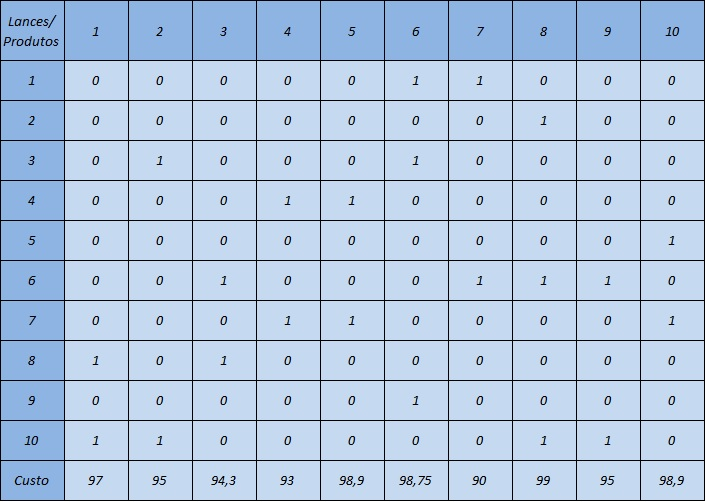
\includegraphics[scale=0.65]{Imagens/Tabela.jpg}
        %     \centering
        %     \caption{Instância}
        % \label{fig:instance}
        % \end{figure} 
	
	    \todo[inline]{Descrever como é a tabela}
	    
	\todo[inline]{Colocar Referência das instâncias!}
	
	\section{Discussão}\label{sec:disc}
	
	\section{Conclusão}\label{sec:concl}
	

\bibliographystyle{unsrt}
\bibliography{referencias.bib}

\end{document}